\documentclass[12pt,fleqn]{article}
\setlength{\parindent}{0pt}
\usepackage{graphicx}
\usepackage{listings}
\usepackage[latin5]{inputenc}
\setlength{\parskip}{8pt}
\setlength{\parsep}{0pt}
\setlength{\headsep}{0pt}
\setlength{\topskip}{0pt}
\setlength{\topmargin}{0pt}
\setlength{\topsep}{0pt}
\setlength{\partopsep}{0pt}
\setlength{\mathindent}{0cm}

\begin{document}
MIT OCW Cok Degiskenli Calculus - Ders 13

Lagrange Carpanlari (Multipliers)

Amac yine $f(x,y,z)$ gibi birden fazla degisken iceren bir fonksiyonu
maksimize etmek, degisik olan, $x,y,z$ degiskenlerinin birbirinden bagimsiz
ol\textbf{ma}masi. Bu degiskenlerin arasindaki iliski $g(x,y,z)=c$ gibi bir
fonksiyon tarafindan gosteriliyor olabilir, $c$ bir sabittir. Yani
$f(x,y,z)$'i minimize ya da maksimize ediyoruz ve bunu sadece $g(x,y,z)=c$
sartina / sinirlama ifadesine (constraint) uyan $x,y,z$ degerleri icin
yapiyoruz.

Bunun icin hangi teknigi kullaniriz? Yollardan biri, eger sinirlama ifadesi
basit ise, belki bir degiskeni cebirsel olarak cozmek (digerleri
baglaminda ifade ederek), sonra geri $f$'e sokariz, boylece klasik bir min
/ maks problemi elde ederiz, ki o tur bir problemi cozmeyi artik biliyoruz.

Fakat bazen $x,y,z$ degiskenleri icin analitik cozum mumkun olmaz, o zaman
farkli teknikler kullanmamiz gerekir. Bu derste ogrenecegimiz teknikler
bunlar olacak. 

Uygulama baglaminda, Lagrange Carpanlari bizi niye ilgilendiriyor? Belki
fizik, termodinamik dersinde gormussunuzdur, sicaklik, hacim ve basinc
degerleri vardir, ve bu degerler birbirinden bagimsiz
degildir. Termodinamikte $PV=nRT$ denklemi vardir, gerci burada analitik
olarak basitlestirme yapabilirdik, ama bazi sartlarda tum degiskenleri
oldugu gibi tutmayi isteyebiliriz. 

Simdiye kadar min / maks problemleri icin gordugumuz kritik nokta bulma
tekniklerinin burada ise yarayamacagini hemen belirtelim. O kritik noktalar
$g(x,y,z)=c$ sinirlama ifadesini tatmin etmiyor olabilirler. Baska bir seye
ihtiyacimiz var. 

Ornek

Hiperbol $xy =3$ uzerinde olan ve orijine en yakin noktayi bul. 

Aslinda bu soruyu temel geometri kullanarak cozebiliriz, fakat burada
Lagrange Carpanlari kullanarak cozecegiz, cunku iyi bir ornek. 

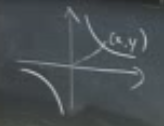
\includegraphics[height=2cm]{13_1.png}

Neyi minimize edelim? Mesela $f(x,y) = \sqrt{x^2 + y^2}$ olur mu? Olabilir,
ama karekok ifadesinden kurtulursak daha iyi olur. 

O zaman

\[ min \ f(x,y) = x^2 + y^2 \]

\[ ki, \ xy = 3  \]

Yani sinirlama ifadesini $g(x,y) = xy$ olarak sectik. 

Grafige bakalim. Yuvarlaklar $f(x,y)$ konturlari, yesil okla gosterilen
mesela $f(x,y) = 20$ konturu. Bu kontur ust sag kose ve sol alt kosede
gosterilen hiperbolu kesiyor mu? Evet. Fakat $f(x,y) = 10$, vs. diyerek
daha kucuk yuvarlaklar elde edebilir miyim? Evet. Fakat bir noktadan sonra
bu halkalar hiperbolu kesmeyecektir. 

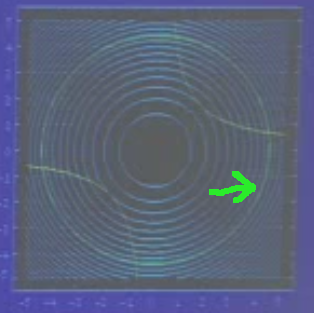
\includegraphics[height=4cm]{13_2.png}

Aradigimiz $x,y$ degerleri hiperbole teget olan, olabilecek en kucuk
yuvarlak.

Cozum icin tegetlik kavramindan faydalanabiliriz. Eger olabilecek en
minimal $f$, her iki fonksiyonun kesit egrilerinin teget oldugu noktada
ise, bu noktayi bulmaya ugrasabilirim. 

Iki kesit egrisi birbirine teget ise, onlarin teget duzlemi paraleldir,
eger oyleyse, bu duzlemlerin normalleri birbirine paralel olmalidir. 

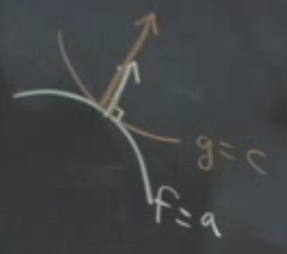
\includegraphics[height=4cm]{13_3.png}

Bu normallerin ayni boyda olmasi gerekmez, yukaridaki gibi, ama paralel
olmalari gerekir. Bu durumda 

\[ \nabla f // \nabla g \]

ifadesi dogru olmalidir, yani $f$'in gradyani $g$'nin gradyanina
paraleldir. Bazi ornekler [hocanin kullandigi program mouse ile tiklanan
yerde (mavi nokta) her iki fonksiyonun gradyanini hemen grafikliyebiliyor,
alttaki resimler birkac ornek noktada yapilan tiklamalar]. 

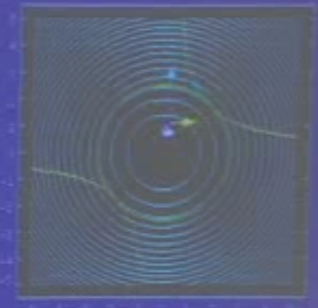
\includegraphics[height=3cm]{13_4.png}

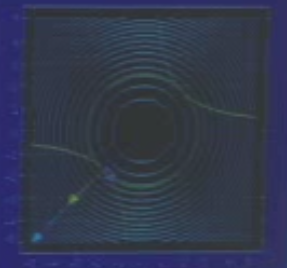
\includegraphics[height=3cm]{13_6.png}

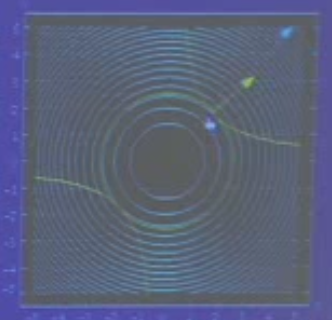
\includegraphics[height=3cm]{13_5.png}

Goruldugu gibi minimal noktalarin birinde (ustteki son resim) gradyanlar
paralel. 

Cebirsel olarak dusunursek: vektorler ne zaman birbirine paralel olur?
Birbirlerinin kati olduklari zaman. Yani su sekilde bir ifadeyi
yazabildigimiz zaman

\[ \nabla f = \lambda \nabla g \]

ki $\lambda$ bir sabit. 

Gradyanlar ayni yonu gostermiyor olabilir, bu durumu $\lambda$'nin negatif
olup olmamasi halledecektir.

Yani aradigimiz $xy$ uzerinde sayisal deger $\lambda$ uzerinden $\nabla f =
\lambda \nabla g $ 
ifadesinin dogru oldugu bir nokta, ve $\lambda$ degeri
ariyoruz (unutmayalim, gradyanlar belli $x,y$ degerleri uzerinden
alinir). Yani 2 degisken iceren sinirlama ifadesi $g(x,y)=c$ iceren bir min /
maks problemi yerine, bir denklem sistemi geciriyoruz. Bu sistem nedir?
Yani ustteki gradyan formuludur, o da su sisteme donusur:

\[ f_x = \lambda g_x \]

\[ f_y = \lambda g_y \]

Oyle degil mi? Cunku $\nabla f$ ve $\nabla g$ birer vektordur, 

\[ 
\nabla f =
\left[\begin{array}{r}
f_x \\
f_y
\end{array}\right], \ \ 
\nabla g =
\left[\begin{array}{r}
g_x \\
g_y
\end{array}\right]
 \]

O zaman iki ustteki denklem sistemi suradan ileri gelmektedir

\[ 
\left[\begin{array}{r}
f_x \\
f_y
\end{array}\right]  = 
\lambda
\left[\begin{array}{r}
g_x \\
g_y
\end{array}\right]
 \]

Fakat hala eksik bir sey var. Elimizde $x,y,\lambda$ bilinmeyenleri var,
ama sadece iki tane formul var. Eksik olan $g(x,y) = c$, cunku $x,y$
birbirinden bagimsiz degil ve $g$ uzerinden baglantililar. Simdi oldu. 3
formul soyle:

\[ f_x = \lambda g_x \]

\[ f_y = \lambda g_y \]

\[ g(x,y) = c \]

Ornegimiz 

\[ f(x,y) = x^2 + y^2 \]

\[ g(x,y) = xy  \]

uzerinde uygularsak

\[ 2x = \lambda y \]

\[ 2y = \lambda x \]

\[ xy = 3 \]

Bu sistemi cozmemiz gerekiyor. Yanliz sunu soyleyelim, bu sistemi cozmenin
genel (hep isleyen) bir yontemi yoktur. Cozum bazen cok basittir, bazen
zordur, bazen sadece sayisal / numerik / hesapsal acidan cozulebilir
(bilgisayar ile). Bu ornekte kolay. 

\[ 2x - \lambda y = 0\]

\[ 2y= \lambda x = 0 \]

\[ xy = 3 \]

Matris formuna koyarsak

\[ 
\left[\begin{array}{rr}
2 & -\lambda \\
\lambda & -2
\end{array}\right]
\left[\begin{array}{r}
x \\ y
\end{array}\right]
=
\left[\begin{array}{r}
0 \\ 0
\end{array}\right]
 \]

En basit cozum $x=0,y=0$ sinirlama ifadesi $xy=3$'u cozmez. Diger cozum ne
zaman ortaya cikar? Eger matrisin determinanti sifir ise. 

\[ 
\left|\begin{array}{rr}
2 & -\lambda \\
\lambda & -2
\end{array}\right| = -4 + \lambda^2 = 0
 \]

\[ <=> \lambda^2 = 4 \]

\[ <=> \lambda = \pm 2 \]

Elimizde iki durum var. $\lambda$ ya 2, ya da -2. 

1. $\lambda = 2$ durumunda

\[ x = y \]

\[ x^2 = 3 \]

O zaman

$(x,y)$ = $(\sqrt{3}, \sqrt{3})$ ya da $(-\sqrt{3}, -\sqrt{3})$ 

2. $\lambda = -2$ durumunda

\[ x = -y \]

\[ -x^2 = 3 \]

Bu durumda cozum yoktur (karesi alinip eksi ile carpilan hicbir sayi 3
sonucunu vermez). 

Ustteki son iki resime bakinca, $\lambda = 2$'nin dogru oldugunu goruyoruz,
cozum olan iki noktada bir gradyan otekinin hakikaten tam iki kati. 

Bu metot niye isledi? Grafiklere baktik, tegetlik oldugunu gorduk, fakat
bunun niye kesinlikle boyle olmasi gerektigini soylemedik. 

Kisitli ifade gozonune alininca ele gececek bir min / maks noktasinda ve
$g = c$ kesit egrisi boyunca, $f$'in degisim orani $=0$ olmalidir.

Simdi ayni seyi yonsel turev kullanarak soyleyelim. 

$g=c$'e teget olan her $\hat{u}$ icin $df / ds_{|\hat{u}} = 0$ olmali. 

Yani su resme bakarsak

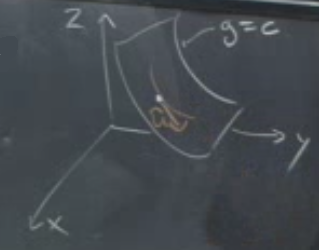
\includegraphics[height=4cm]{13_7.png}

Kesit yuzeyi (ki orada $g=c$) uzerindeki nokta ve o yuzeye teget olan yon
$\hat{u}$ yonunde $f$'in degisimi sifirdir. 

$df / ds_{|\hat{u}}$ formulunun $\nabla f \cdot \hat{u}$ formulune esit oldugunu  biliyoruz. 

O zaman teget olan her $\hat{u}$, $\nabla f$'e dik olmalidir, yani $\hat{u} \perp \nabla f$. 

O zaman $\nabla f$, $g$'nin kesit seviyelerine diktir. 

$g$'nin kesit seviyelerine dik bir baska vektor daha biliyoruz, o 
da $g$'nin kendi gradyani, yani $\nabla g$. 

O zaman $\nabla f // \nabla g$ olmalidir cunku her iki gradyan da $g$'nin
kesit seviyelerine ayni anda diktir. 

Tekrar edelim. Sinirlanmis min, maks noktasinda $g$ kesit seviyesi uzerinde
ilerliyorsak, $f$'in (en azindan birinci derecedeki yaklasiksallamasindaki)
degisimi sifirdir, yani $g=c$'ye teget yondeki herhangi bir $f$ turevi sifir
olmali. Min, maks olmak bu demek. O zaman $g=c$'ye teget olan herhangi bir
$\hat{u}$, $f$'in gradyani $\nabla f$'e dik olmalidir, ve bu da $\nabla f$,
$g$'nin kesit seviyesine dik demektir. 

Yani resimde gordugumuz tekrar soylemis oluyoruz. Her iki kesit seviyesi
kisitlanmis min / maks noktasinda birbirine teget olmali.

UYARI

Bu metot bir cozumun min mi, maks mi oldugunu soylemez. 

Kotu haber: 2. turev testini kullanamayiz. 

Ne yapabiliriz? Elde edilen noktalari $f$'e verip sonuca teker teker
bakariz, birbirleri ile karsilastiriz. Mesela ustteki ornekten elde
ettigimiz degerler minimum'dur, maks bu problemde sonsuzluktadir.

Zor Ornek

Diyelim ki bir piramit insa etmek istiyoruz, hacim ve ucgensel taban bize
veriliyor. Amac, tum dis yuzey alanini minimize etmek. 

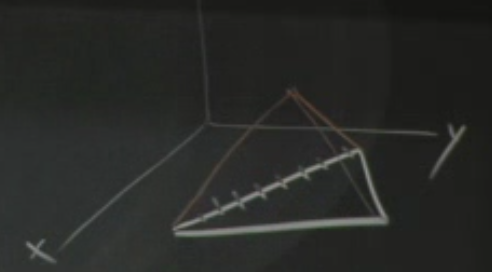
\includegraphics[height=3cm]{13_8.png}

Cozum icin bulmamiz gereken piramidin en ust noktasi. Degisik yerlerde
olabilecek, ve nerede olduguna gore hacimin, alanin degisebilecegi
elimizdeki ayar noktasi orasi. Hacim formulu

Hacim = $\frac{1}{3}$ Baz alani $\times$ yukseklik

Hacmi ve baz alani sabitlediysek, o zaman formulde geri kalan yukseklik te
sabitlenmis demektir. Minimize ederken onun uzerinde oynayamayiz. O zaman
ust nokta sadece xy duzlemine paralel olarak saga, sola, ileri, geri,
vs. seklinde yer degistirebilir, asagi, yukari cikamaz. 

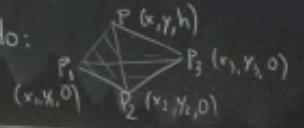
\includegraphics[height=3cm]{13_9.png}

Eger kordinatlari ustteki gibi ortaya cikartsak, ele gecen tum ucgenlerin
alan hesabini vektor capraz carpimi ile hesaplamayi biliyoruz, onlarin
toplamini elde etmeye ugrasabilirdik, vs. Fakat ustteki yontem isleri daha
fazla karistiriyor. Kordinatlari daha iyi temsil edecek bir yontem
gerekiyor bize.

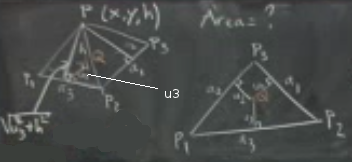
\includegraphics[height=4cm]{13_10.png}

Temsili ustteki gibi yapalim, resimde sagda olan sekil piramidin kusbakisi
goruntusu. Piramit tabaninda bir $Q$ noktasi hayal edelim, $P_1$  ve $P_2$
arasindan $Q$'ye giden uzaklik $u_3$ [resimde iyi cikmadi, biz ekledik],
yuksekligi zaten biliyoruz, $h$. O zaman piramit kenarinda ona tekabul eden
yukseklik $\sqrt{u_3^2 + h^2}$. 

\[ \textrm{Kenar alani } = 
\frac{1}{2}a_1 \sqrt{u_1^2 + h^2} + 
\frac{1}{2}a_2 \sqrt{u_2^2 + h^2} + 
\frac{1}{2}a_3 \sqrt{u_3^2 + h^2} 
 \]

Bu 3 degisken iceren bir fonksiyon, $f(u_1,u_2,u_3)$. 

Uc degiskeni birbiri ile nasil iliskilendiririz? Cunku buyuk bir ihtimalle
bunlar bagimsiz degiskenler degiller.

Eger ust resimdeki sag sekle bakarsak, ve baz alanini uc parcaya bolersek,
elde ettigimiz

\[ \textrm{Baz alani } = 
\frac{1}{2}a_1u_1 +  
\frac{1}{2}a_2u_2 +  
\frac{1}{2}a_3u_3
\]

formuludur. Bu formul kisitlama ifadem, yani bu problemnin $g$'si. Kenar
alani formulu de $f$'im. 

Lagrange

\[ \nabla f = \lambda \nabla g \]

\[ \frac{\partial f}{\partial u_1} =
\frac{1}{2}a_1 \frac{u_1}{\sqrt{u_1^2 + h^2}} = 
\lambda \frac{1}{2}a_1
\]

$1/2a_1$'ler iptal olur

\[
\frac{\partial f}{\partial u_1} =
\frac{u_1}{\sqrt{u_1^2 + h^2}} = \lambda 
\]

Digerleri benzer sekilde

\[
\frac{\partial f}{\partial u_2} =
\frac{u_2}{\sqrt{u_2^2 + h^2}} = \lambda 
\]

\[
\frac{\partial f}{\partial u_3} =
\frac{u_3}{\sqrt{u_3^2 + h^2}} = \lambda 
\]

Son uc formulun ucu de $\lambda$'ya esit, o zaman uc formul birbirine
esit. Bu mantigi izlersek, $u_1 = u_2 = u_3$ olmasi gerektigi sonucuna da
variriz. 

O zaman $Q$ noktasi her kenardan esit uzaklikta, tam ortada (incenter)
olmali. 









\end{document}
